\subsection{Mapping}
\label{sec:models/kf/mapping}
In the mapping problem, we assume we don't have the knowledge of the map $\vec M$ (described in subsection \ref{subsec:models/kf/localisation}), but know the vehicle states $\vec x_1, \dotsc, \vec x_T$ exactly. We want to figure out $\vec M$. The graphical model is as follows
\begin{figure}[!htb]
\centering
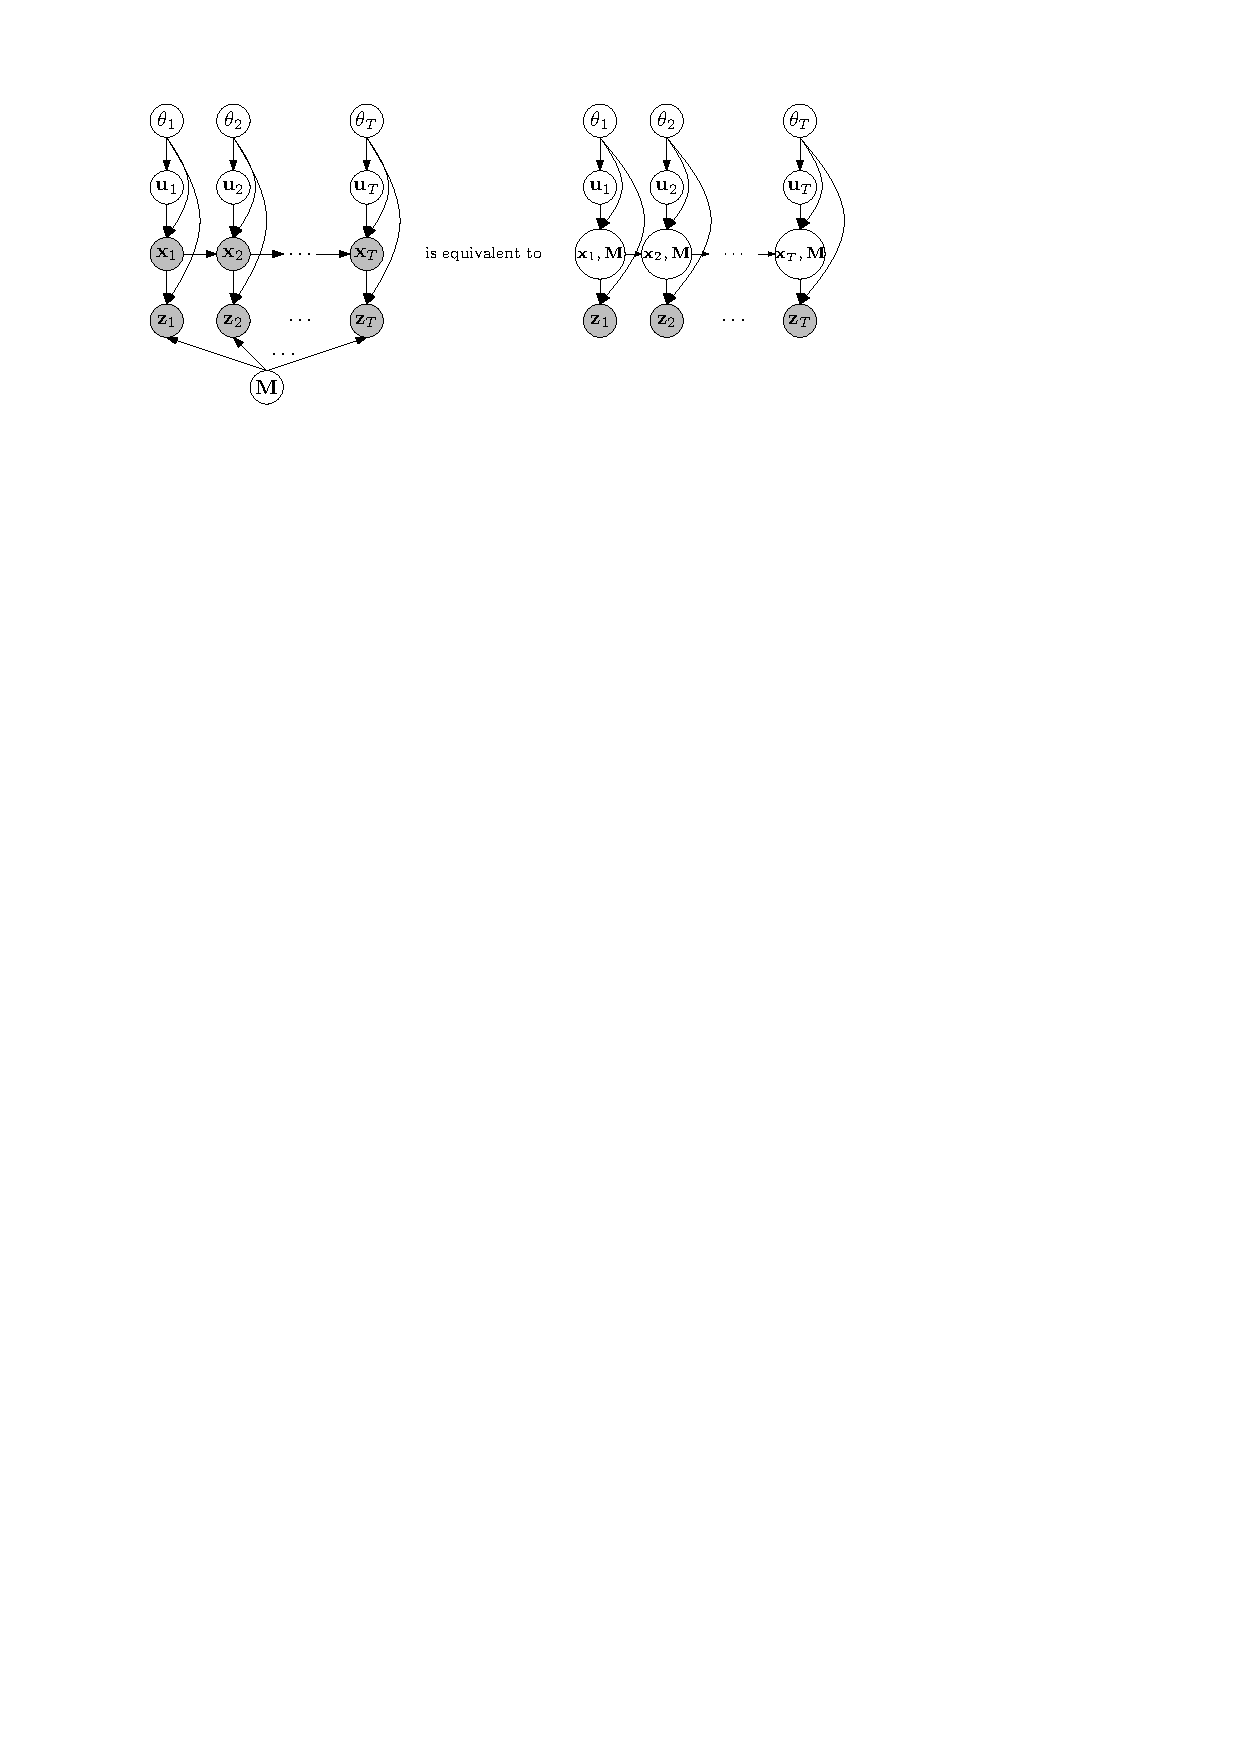
\includegraphics[scale=1]{models/kf/figures/kf-map}
\caption{Probabilistic Graphical Model for the Kalman Filter for Mapping.}
\label{fig:models/kf/figures/kf-map}
\end{figure}

on the left, we shade $\vec x_1, \dotsc, \vec x_T$ and $\vec z_1, \dotsc, \vec z_T$ to signify that they are observed variables. On the right, we group the $\vec x$'s and $\vec M$ together. We call these random variables, for $t = 1, \dotsc, T$
\begin{equation}
	\vec x_t^\ast =
		\begin{bmatrix}
			\vec x_t \\
			\vec M
		\end{bmatrix}
\end{equation}
Since these random variables are only ``half-observed'', we don't shade them.

The model can be described, for $t = 1, \dotsc, T$, by the following equations:
\begin{align}
	\vec x_t^\ast 	&= \vec g^\ast(\vec x_{t - 1}^\ast, \vec u_t) + \vec \epsilon_t^\ast \\
	\vec z_t 		&= \vec h^\ast(\vec x_t^\ast, \vec u_t) + \vec \delta_t^\ast
\end{align}
We need to characterise $\vec g^\ast(\vec x^\ast, \vec u)$, $\vec \epsilon_t^\ast$, $\vec h^\ast(\vec x^\ast, \vec u)$, and $\vec \delta_t^\ast$ to describe the EKF algorithm fully.

